\documentclass[10pt]{article}
\usepackage[a4paper,left=1.22cm,right=1.22cm,top=1.0cm,bottom=0.9cm]{geometry}
\usepackage{fontspec}
\setmainfont{Inter}[RawFeature={-calt},UprightFont=*-Regular,BoldFont=*-SemiBold,ItalicFont=*-Italic,BoldItalicFont=*-SemiBoldItalic]
\setsansfont{Inter}[RawFeature={-calt},UprightFont=*-Regular,BoldFont=*-SemiBold,ItalicFont=*-Italic]
\usepackage{unicode-math}
\setmathfont{Latin Modern Math}
\usepackage{graphicx,xcolor,tabularx,booktabs,array,colortbl,enumitem,tikz,multicol}
\usepackage[most]{tcolorbox}
\usepackage[hidelinks]{hyperref}
\usetikzlibrary{positioning,arrows.meta}
\definecolor{fmblue}{HTML}{2F80D5}
\definecolor{fmred}{HTML}{D64545}
\definecolor{fmpale}{HTML}{EEF4FC}
\definecolor{fmgrey}{HTML}{6B6B6B}
\definecolor{fmrow}{HTML}{EEF2F8}
\pagestyle{empty}
\setlength{\parindent}{0pt}
\setlength{\parskip}{1.5pt}
\setlist[itemize]{leftmargin=9pt,itemsep=0.6pt,topsep=1pt,parsep=0pt,label=\textbullet}
\newcommand{\body}{\fontsize{8.4}{10.1}\selectfont}
\newcommand{\head}[2]{\par\vspace{3pt}{\fontsize{9.6}{11}\selectfont\color{fmblue}\textbf{#1}\ifx&#2&\else: #2\fi}\par\vspace{1.5pt}}
\newcommand{\up}[1]{\textcolor{fmblue}{\textbf{#1}}}
\newcommand{\dn}[1]{\textcolor{fmred}{#1}}
\newcommand{\kpi}[3]{\begin{tcolorbox}[enhanced,width=\linewidth,colback=white,colframe=black!25,arc=2pt,boxrule=0.4pt,left=3pt,right=2pt,top=2pt,bottom=2pt]{\fontsize{15}{16}\selectfont\textbf{#1}}\\[-1pt]{\fontsize{7.6}{8.5}\selectfont\textbf{#2}}\\[-1pt]{\fontsize{6.6}{7.5}\selectfont\color{fmgrey}#3}\end{tcolorbox}}
\newcolumntype{R}{>{\raggedleft\arraybackslash}X}
\newcolumntype{L}{>{\raggedright\arraybackslash}X}

\begin{document}
\body
% ---------------------------------------------------------------- header
{\fontsize{7.4}{9}\selectfont\color{fmblue}\textbf{SYSTEMATIC EQUITY MARKET-NEUTRAL STOCK SELECTION (OPEN-SOURCE PROOF OF CONCEPT)}\hfill\textcolor{black}{\textbf{KHALED BAHA}}}\par\vspace{2pt}
{\fontsize{19}{21}\selectfont\color{fmblue}\textbf{First-Mover Flow (FMF-N)}}\par\vspace{1pt}
{\fontsize{10.5}{12}\selectfont\color{fmblue}Zero-beta stock selection for concentrated equity portfolios, from \emph{who} revises first and \emph{when}}\par
\vspace{2pt}{\color{fmblue}\rule{\linewidth}{0.6pt}}\par\vspace{2pt}

% ---------------------------------------------------------------- problem | idea
\begin{minipage}[t]{0.488\linewidth}
\head{THE BUSINESS PROBLEM}{}
Tech, thematic and high-conviction funds, and QIS baskets on narrow universes, hold \textbf{concentrated portfolios}. With 10–30 names breadth is very low, so real stock-picking skill is hard to see in the statistics, and most signals end up as beta or momentum under another name. A regime filter that adds net exposure in a bull market then looks like skill. My first-generation strategy reached a Calmar of 1.77, yet its timing leg did worse than a \emph{static} beta of the same size.
\smallskip
What I was after is a stock-selection alpha that is \emph{independent of the market}, lifts the Calmar ratio by itself, and fits into the funds and indices desks already run.
\end{minipage}\hfill
\begin{minipage}[t]{0.488\linewidth}
\head{THE IDEA}{}
Sell-side analysts revise at different times. \textbf{First movers} revise on an earnings day or after ≥10 sessions without a revision on the stock, the market takes weeks to absorb their information. \textbf{Herders} follow an earnings cluster 3–15 sessions later, in its direction, when the move is mostly done. The \textbf{leader-minus-herd} signal (LMH) is the difference of the two.
\begin{itemize}
\item IC of leaders \up{+0.066}, of herders \dn{−0.084}
\item only one of 18 candidates with power beyond four price factors (Fama–MacBeth $t$ = 2.46)
\item \textbf{replicates on a never-seen period}: IC \up{0.096}, $p$ = 0.042, 0.105 on the 20 names not used in development
\end{itemize}
LMH enters an equal-weight rank composite with three revision-breadth signals. No weights are fitted.
\end{minipage}

% ---------------------------------------------------------------- research path
\head{THE RESEARCH PATH}{FROM REGIME TIMING TO SELECTION ALPHA}
\begin{tcbraster}[raster columns=3,raster equal height,raster column skip=14pt,raster left skip=0pt,raster right skip=0pt]
\begin{tcolorbox}[colback=white,colframe=black!25,arc=2pt,boxrule=0.4pt,left=4pt,right=4pt,top=2pt,bottom=2pt]
\textbf{Gen 1: Regime-Timed Breadth (RTB)}\\
Classic revision breadth with GJR-GARCH sizing and an HMM/trend tilt of net exposure. Point in time walk-forward. \textbf{Calmar 1.77} in development and 1.65 in the holdout.
\end{tcolorbox}
\begin{tcolorbox}[colback=white,colframe=fmred,arc=2pt,boxrule=0.5pt,left=4pt,right=4pt,top=2pt,bottom=2pt]
\textcolor{fmred}{\textbf{Diagnosis: beta camouflage}}\\
Selection book alone: Sharpe 0.63, Calmar 0.36, placebo $p$ 0.08–0.14. A \emph{constant} 0.2 beta did better than the timing leg (Calmar 1.82). Without beta little stock-picking alpha remained.
\end{tcolorbox}
\begin{tcolorbox}[colback=fmpale,colframe=fmblue,arc=2pt,boxrule=0.5pt,left=4pt,right=4pt,top=2pt,bottom=2pt]
\textcolor{fmblue}{\textbf{Gen 2: First-Mover Flow (FMF-N, FMF-B20)}}\\
New signal (leader minus herd), 42-session tranches, zero beta. Selection Sharpe 0.63 to 0.98, Calmar 0.36 to 0.79, turnover 10.8x to 2.1x, placebo $p$ = 0.022.
\end{tcolorbox}
\end{tcbraster}

% ---------------------------------------------------------------- KPI tiles
\vspace{3pt}
{\fontsize{6.9}{8}\selectfont\color{fmgrey}\textbf{IN SAMPLE 2017–2021} (10 US large caps development + holdout)\hfill\textbf{OUT OF SAMPLE 2024–2026} (30 stocks never-seen period frozen pre-registered)}\par\vspace{1pt}
\begin{tcbraster}[raster columns=8,raster equal height,raster column skip=3pt,raster left skip=0pt,raster right skip=0pt]
\kpi{1.13}{Sharpe, net}{holdout 1.33}
\kpi{0.78}{Calmar}{Gen 1 book 0.53}
\kpi{−0.02}{Beta}{dollar-neutral}
\kpi{7.4\%}{4-factor alpha}{$t$ = 2.98}
\kpi{1.05}{Sharpe, net}{both halves > 0}
\kpi{1.32}{Calmar}{max DD −8.0\%}
\kpi{11.4\%}{CAPM alpha}{$t$ = 2.04}
\kpi{\#2\,/\,14}{vs institutional}{on both metrics}
\end{tcbraster}

\vspace{2pt}
\centerline{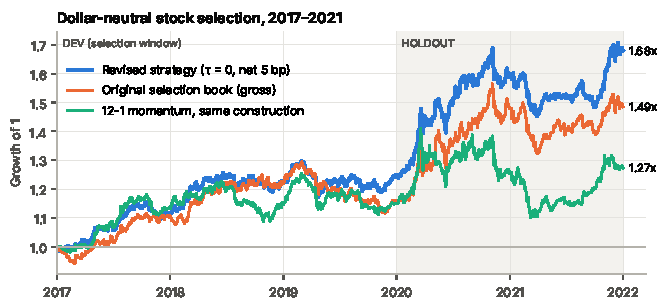
\includegraphics[width=0.66\linewidth]{fig/equity.pdf}}

% ---------------------------------------------------------------- toolkit table
\head{OUTPERFORMANCE AGAINST THE INSTITUTIONAL TOOLKIT}{SAME CONSTRUCTION NET OF 5\,BP}
{\fontsize{7.8}{9.3}\selectfont
\begin{tabularx}{\linewidth}{@{}p{0.36\linewidth}RRRR@{\hspace{14pt}}RR@{}}
\toprule
 & \multicolumn{4}{c}{\textbf{In sample 2017–2021}} & \multicolumn{2}{c}{\textbf{Never-seen period 2024–26}}\\
\cmidrule(lr){2-5}\cmidrule(l){6-7}
 & Sharpe & Calmar & Max DD & Corr. FMF & Sharpe & Calmar\\
\midrule
\rowcolor{fmrow}\textbf{First-Mover Flow (FMF-N)} & \textbf{1.13} & \textbf{0.78} & −14.1\% & 1.00 & \textbf{1.05} & \textbf{1.32}\\
12-1 momentum (Jegadeesh–Titman) & 0.50 & 0.23 & −21.8\% & 0.71 & 0.60 & 0.62\\
Residual momentum (Blitz et al.) & 0.17 & 0.05 & −24.1\% & 0.64 & 0.56 & 0.54\\
Low volatility & 0.56 & 0.37 & −13.6\% & 0.04 & −0.39 & −0.17\\
Betting-against-beta & −0.15 & −0.07 & −32.2\% & 0.10 & −0.94 & −0.32\\
Consensus target-price upside & 0.38 & 0.24 & −12.1\% & −0.38 & 0.11 & 0.05\\
Classic revision breadth & 0.92 & 0.58 & −15.5\% & 0.95 & 0.98 & 1.16\\
Multi-factor: momentum + low vol + reversal & 0.81 & 0.42 & −14.3\% & 0.44 & −0.00 & −0.01\\
\midrule
First-Mover Flow + 0.2 beta budget (FMF-B20) & 1.62 & \textbf{1.66} & −10.8\% & – & 1.49$^\dagger$ & \textbf{2.43}$^\dagger$\\
Regime-Timed Breadth (RTB Gen 1) & 1.48 & 1.39 & −13.6\% & – & – & –\\
Equal-weight long-only market (beta 1) & 1.28 & 0.87 & −38.1\% & −0.02 & 1.14 & 0.94\\
\bottomrule
\end{tabularx}\par\vspace{1pt}
{\fontsize{7.2}{8.6}\selectfont\color{fmgrey}FMF-N is first of 14 cross-sectional books in sample and second out of sample after target-price momentum (Sharpe 1.14). Blending 50/50 with FMF-N raises the Sharpe of 16/18 institutional books in sample and 16/16 out of sample. Every choice was made on 2017–19 data. $^\dagger$FMF-B20 out of sample is exploratory, its 0.2 budget was set in development but is not in the pre-registration.}}

\newpage
% ================================================================ PAGE 2
\head{HOW IT WORKS}{SIGNAL AND CONSTRUCTION AND RISK LOGIC}
\begin{center}
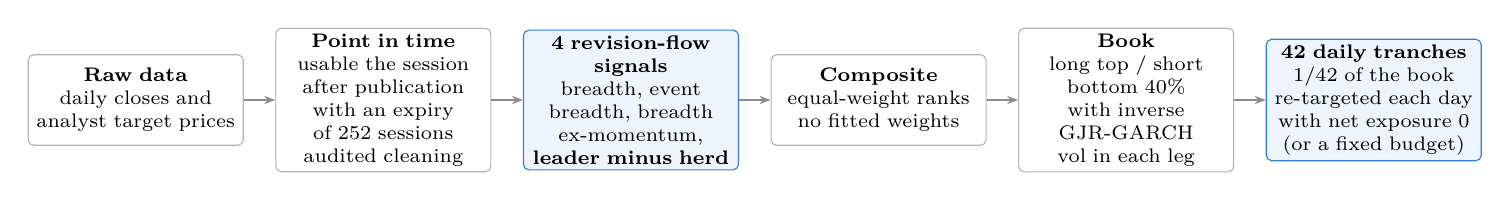
\begin{tikzpicture}[node distance=4.0mm,
 box/.style={draw=black!30,rounded corners=2pt,align=center,minimum height=11.5mm,text width=25.9mm,font=\fontsize{7.1}{8.3}\selectfont,execute at begin node={\hyphenpenalty=10000\exhyphenpenalty=10000},inner sep=2pt},
 hl/.style={box,draw=fmblue,fill=fmpale}, arr/.style={-{Stealth[length=4pt]},black!45}]
\node[box] (a) {\textbf{Raw data}\\daily closes and \\analyst target prices};
\node[box,right=of a] (b) {\textbf{Point in time}\\usable the session after publication with an expiry of 252 sessions  audited cleaning};
\node[hl,right=of b] (c) {\textbf{4 revision-flow signals}\\breadth, event breadth, breadth ex-momentum, \textbf{leader minus herd}};
\node[box,right=of c] (d) {\textbf{Composite}\\equal-weight ranks no fitted weights};
\node[box,right=of d] (e) {\textbf{Book}\\long top / short bottom 40\% with inverse GJR-GARCH vol in each leg};
\node[hl,right=of e] (f) {\textbf{42 daily tranches}\\1/42 of the book re-targeted each day with net exposure 0 (or a fixed budget)};
\foreach \x/\y in {a/b,b/c,c/d,d/e,e/f} \draw[arr] (\x) -- (\y);
\end{tikzpicture}
\end{center}
\vspace{-2pt}
\begin{minipage}[t]{0.5\linewidth}
\head{RISK-MANAGEMENT LOGIC}{}
The book is dollar-neutral every day. Market exposure, if wanted, is a constant beta budget set in advance and never timed. FMF-B20 (net 0.2) has a Calmar of 1.66 over 2017–21, against 1.39 for the regime-timed predecessor, with a max drawdown of −10.8\%. Inverse GJR-GARCH-$t$ weights scale down the names whose drawdowns would dominate.\par\smallskip
Information from revisions builds over several weeks (IC 0.026 at 1 day, 0.109 at 21), so I trade in overlapping tranches. They remove rebalancing-date luck: with one weekly rebalance date the same signal has a Sharpe between 0.34 and 0.71. Turnover is 2.1–2.7x a year, against 10.8x before. All results are net of 5\,bp per unit traded (Sharpe 1.11 at 10\,bp), and the universe is liquid large caps.
\end{minipage}\hfill
\begin{minipage}[t]{0.46\linewidth}
\head{CRISIS BEHAVIOUR}{CUMULATIVE RETURN, \%}
{\fontsize{7.9}{9.4}\selectfont\setlength{\tabcolsep}{3pt}
\begin{tabularx}{\linewidth}{@{}>{\raggedright\arraybackslash}p{0.37\linewidth}RRR@{}}
 & COVID crash & Vaccine rally & Growth sell-off\\
 & {\color{fmgrey}\mbox{Feb–Mar 20}} & {\color{fmgrey}Nov 20} & {\color{fmgrey}\mbox{Feb–Mar 21}}\\
\midrule
\rowcolor{fmrow}\textbf{FMF-N} & \textbf{+12.0} & \textbf{−5.8} & \textbf{−7.1}\\
12-1 momentum & +12.2 & −8.2 & −10.5\\
Betting-against-beta & −15.2 & −1.0 & −1.7\\
Trend following (CTA) & −18.9 & −3.5 & −12.1\\
Equal-weight market & −35.5 & +6.9 & −9.4\\
\bottomrule
\end{tabularx}}
\end{minipage}

\head{NINE OBJECTIONS AN INVESTMENT COMMITTEE WOULD RAISE}{}
{\fontsize{7.5}{8.9}\selectfont
\begin{tabularx}{\linewidth}{@{}>{\raggedright\arraybackslash}p{0.21\linewidth}>{\raggedright\arraybackslash}p{0.25\linewidth}>{\raggedright\arraybackslash}X@{}}
\toprule
\textbf{Objection} & \textbf{Test} & \textbf{Result}\\
\midrule
“Hindsight universe: it is just long the winners” & Causal split into static tilt and timing books (Lo 2008) & \up{Timing} earns Sharpe 1.04 ($t$ 2.41), never-seen 1.33 ($t$ 2.21). Static tilt: −0.49.\\
“Close-of-day fills and free shorts are fantasy” & 0–2 day delay × 0–200\,bp borrow × 0–30\,bp costs & Sharpe 1.06 at 1 day, 100\,bp, 10\,bp, breakeven cost \up{234\,bp} per unit traded.\\
“Dollar-neutral is not beta-neutral” & Separate up- and down-market betas, weekly & Down-market beta −0.07 ($t$ −1.24), never-seen −0.01.\\
“Overlapping tranches smooth the P\&L” & Lo (2002) autocorrelation-adjusted Sharpe & 1.06 in both samples (lag-1 autocorrelation 0.04).\\
“You chose the parameters that work” & Multiverse of about 300 specifications (incl. quarterly expiry) & \up{99\%} positive (97\% out of sample), selection-free ensemble Sharpe 0.92.\\
“The new signal adds nothing to breadth” & Same book without leader-minus-herd, block bootstrap & +0.28 Sharpe ($p$ 0.028), out of sample +0.30, pooled $P(>0)$ 0.94.\\
“Beating the toolkit is cherry-picking.” & Romano–Wolf vs 16 books, reverse SPA test & No comparable beats FMF-N (SPA $p$ 0.86 / 0.86).\\
“Ten stocks prove nothing” & Bayesian meta-analysis of 3 non-overlapping samples & $P$(signal works in the \textbf{next} universe) = \up{0.96}, Stouffer $p$ = 0.0022.\\
“One history, one drawdown” & Diffusion-FHS generator (classifier score 0.014, 0 = indistinguishable) & 5-year median Calmar 0.70, 5\% max DD −34\% \dn{momentum crashes} are the binding stress.\\
\bottomrule
\end{tabularx}}

\vspace{2pt}
\noindent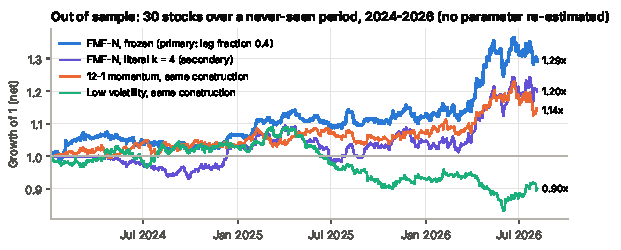
\includegraphics[height=3.55cm]{fig/oos.pdf}\hfill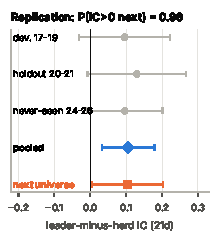
\includegraphics[height=3.55cm]{fig/replication.pdf}\hfill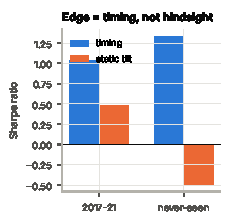
\includegraphics[height=3.55cm]{fig/timing.pdf}

\vspace{3pt}
\begin{minipage}[t]{0.47\linewidth}\vspace{0pt}
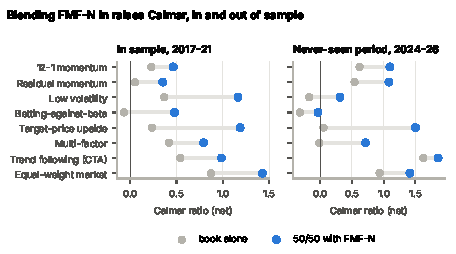
\includegraphics[width=0.9\linewidth]{fig/blend.pdf}
\end{minipage}\hfill
\begin{minipage}[t]{0.47\linewidth}\vspace{0pt}
\head{WHO IT IS FOR}{}
\begin{itemize}
\item \textbf{PMs} of concentrated books get a zero-beta selection sleeve, with today's book, a trade list, a risk report and a signal monitor.
\item \textbf{QIS structurers} get a rules-based index (excess return, vol target, fees, and a rulebook generated from the parameters). In a 50/50 blend it raised the Calmar of every price-factor index tested.
\item \textbf{Quant researchers} get a signal registry, a multiverse, Bayesian and snooping-robust tests and generative stress tests, all of which run on their own data.
\end{itemize}
\end{minipage}

\head{RIGOUR AND LIMITS}{}
Point in time and truncation-tested. Out-of-sample rules were hashed before any result was computed and more than fifty failed ideas are documented. Deflated over every configuration tried the development Sharpe alone is not conclusive (DSR 0.18–0.38) and no single short window is significant once the whole family of specifications is counted. The evidence is the replication over three non-overlapping periods. Ten of the 30 out-of-sample names are development names the other 20 alone give a Sharpe of 0.80. \textbf{Code:} \texttt{fmflow} 100+ tests, 11 notebooks, Docker, it reproduces the research notebook's results.

\vspace{3pt}
{\fontsize{7.1}{8.6}\selectfont\color{fmgrey}Khaled Baha • Khaled.Cheikh.Baha@gmail.com • github.com/bahakh19/first-mover-flow • Paper: “Who Revises First? Analyst Revision Flow and Zero-Beta Stock Selection in Concentrated Equity Portfolios”. Past performance, in or out of sample, does not guarantee future results.}
\end{document}
